%!TEX encoding = UTF-8 Unicode

\documentclass[11pt,largemargins]{homework}
\usepackage[utf8]{inputenc}
\usepackage{amsmath}
\usepackage{tikz}


\newcommand{\hwname}{ENSA-Safi}
\newcommand{\hwemail}{}
\newcommand{\hwtype}{Travaux Dirigés}
\newcommand{\hwnum}{2}
\newcommand{\hwclass}{Probabilité:}
\newcommand{\hwlecture}{3}
\newcommand{\hwsection}{Z}



\begin{document}
\maketitle

% Probabilite conditionelle simple {{{ %
\question*{Probabilité Conditionnelle 1}
Les assertions suivantes sont elles vrai?(Justifier votre réponse)

\begin{enumerate}
    \item Si l'espace des états $\Omega$ est fini et avec un loi de probabilité
        \textbf{uniforme}\footnote {tous les évènements sont équiprobables}. Alors si $B \neq 0$, la probabilité conditionnelle sur
        $\mathbf{B}$ est aussi un loi discrète uniforme.

    \item Si l'espace des états $\Omega$ est fini et avec un loi de probabilité
        \textbf{uniforme}. Alors si $B \neq 0$, la probabilité conditionnelle sur
        $\mathbf{\Omega}$ est aussi un loi discrète uniforme.
\end{enumerate}

% }}} Probabilite conditionelle simple %
% Probabilite conditionelle problem {{{ %
\question*{Probabilité Conditionnelle 2}

On lance deux  dé équilibre a $\mathbf{6}$ faces. Tous les $\mathbf{36}$
résultats sont équiprobables.\\

\begin{arabicparts}
    \item Calculer la probabilité qu'on obtient un \textbf{double}(i.e Les deux
    faces possèdent le même nombre).
\item Étant donné que la sommes des deux dès est inférieure ou
    égale$\mathbf{4}$, calculer la probabilité conditionnelle qu'on obtient un
    double.

\item Calculer la probabilité d'obtenir un six dans l'un des deux
    des.\footnote{On peut obtenir deux six}
\item On sait maintenant que les nombres des deux des sont \textbf{différents},
    calculer la probabilité d'obtenir un $6$ dans l'un des deux dès.

\end{arabicparts}

% }}} Probabilite conditionelle problem %
% Total probablity 1 {{{ %
\question*{Loi de probabilité totale}
On suppose qu'on dispose d'un infinité de pièce de monnaie indexés par $i$.
Chaque pièce de monnaie $i$ peut être choisie avec une probabilité
$\mathbf{2^{-i}}$. Un lancé de la pièce $i$ peut donner Pile avec une
probabilité $\mathbf{3^{-i}}$.\\[4pt]


\begin{arabicparts}
    \item On choisi une pièce de monnaie, puis on lance cette pièce. Quelle est
        la probabilité d'obtenir \textbf{Pile}?


        On rappelle que la somme d'une suite géométrique de raison $\alpha$ est 
        \begin{equation*}
            \sum_{i=1}^\infty \alpha^i = \frac{\alpha}{1 - \alpha}, \text{ si }
            \vert \alpha \vert < 1
        \end{equation*}
\end{arabicparts}
% }}} Total probablity 1 %
% Regle de Bayes {{{ %
\question*{Règle de Bayes}
Un test pour une maladie rare peut être correct a $\mathbf{95\%}$. Si une personne est
malade, alors ce test peut le détecter  avec un probabilité $\mathbf{95\%}$. Si
la personne n'est pas malade, le test sera négatif avec une probabilité
$\mathbf{0.95}$. Finalement $\mathbf{0.001}$ de la population peuvent être malade.

\begin{arabicparts}
    \item Calculer la probabilité qu'une personne  choisie aléatoirement est testé positive.
    \item Étant donne que cette personne est testé positive, quelle est la
        probabilité qu'elle soit vraiment malade?
\end{arabicparts}

% }}} Regle de Bayes %
% Independence {{{ %
\question*{Indépendance}
Vous lancez deux dès a \textbf{cinq} faces. Ces faces sont numérotes de $1$ a
$5$. (Tous les résultats sont équiprobables). On supoose que les deux dès sont
indépendants.

\begin{arabicparts}
    \item On considère l'évènement $A$ "La somme des deux des est $10$"
        \begin{arabicparts}
            \item Est ce que $A$ est indépendant de l'évènement "au moins l'un
                de dès donne $5$".
            \item Est ce que $A$ est indépendant de l'évènement "au moins l'un
                des dès donne $1$"
        \end{arabicparts}
    \item Soit l'évènement $B$ "la somme est $\mathbf{8}$"
        \begin{arabicparts}
            \item Est ce que l'évènement $B$ est indépendant de "Obtenir un
                double"(i.e. Les résultats des deux faces sont égaux).
        \end{arabicparts}

\end{arabicparts}
% }}} Independence %
% Probblem de fiabilité {{{ %
\question*{Problème de fiabilité}

On considère le réseau de télécommunication dans la figure (\ref{fig:network}).
On suppose que chaque lien peut tomber en panne avec \textbf{probabilité p}. On
suppose que les pannes entre les liens sont \textbf{indépendants}.

\begin{figure}[htpb]
    \centering
    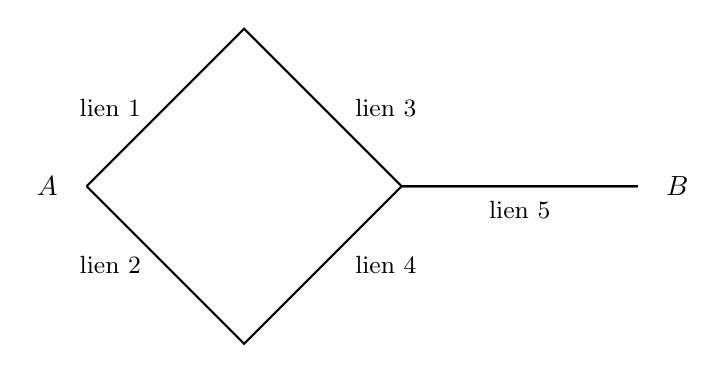
\begin{tikzpicture}
    \path[thick, draw] (0,0) -- (2,2)--(4,0)--(7,0);
    \path[thick, draw] (0,0) -- (2,-2)--(4,0)--(7,0);
    \node (A) at (-.5,0) {$A$};
    \node (B) at (7.5,0) {$B$};

    \node at (0.3,1) {\small lien 1};
    \node at (0.3,-1) {\small lien 2};
    \node at (3.8,1) {\small lien 3};
    \node at (3.8,-1) {\small lien 4};
    \node at (5.5,-.3) {\small lien 5};

    \end{tikzpicture}
    \caption{Réseaux de télécommunication}
    \label{fig:network}
\end{figure}

\begin{arabicparts}
    \item On  suppose que $p = \frac{1}{3}$, calculer la probabilité qu'on
        trouve un lien entre $A$ et $B$ sans aune panne.
    \item Maintenant, on sait qu'il \textbf{seul lien qui est en panne},
        calculer la probabilité de trouver un chemin entre $A$ et $B$.
\end{arabicparts}

% }}} Probblem de fiabilité %
\end{document}
